
\documentclass{article}

\usepackage{graphicx}
\usepackage{booktabs}

\title{AutoRSpec}
\date{2017-04-25}
\author{Dan Shreeve}

\begin{document}

	\pagenumbering{gobble}
	\maketitle
	\newpage
	\tableofcontents
	\newpage
	
	\pagenumbering{arabic}
	\section{Chapter 1: Introduction}
		Filler text, filler text, filler text, filler text, filler text, filler text, filler text, filler text.
	\section{Chapter 2: Literature Review}
		Filler text, filler text, filler text, filler text, filler text, filler text, filler text, filler text.
	\section{Chapter 3: Requirements and Analysis}
		Filler text, filler text, filler text, filler text, filler text, filler text, filler text, filler text.
	\section{Chapter 4: Design}
		Filler text, filler text, filler text, filler text, filler text, filler text, filler text, filler text.
	\section{Chapter 5: Implemention and Design}
		Filler text, filler text, filler text, filler text, filler text, filler text, filler text, filler text.
	\section{Chapter 6: Results and Discussion}
		Filler text, filler text, filler text, filler text, filler text, filler text, filler text, filler text.
	\section{Chapter 7: Conclusions}
		Filler text, filler text, filler text, filler text, filler text, filler text, filler text, filler text.

	\bibliography{bibliography}
	\bibliographystyle{ieeetr}
\end{document}
\par Software disasters can be caused by poor testing practices,\cite{mcquaid2012software} if the correct testing procedures practices were in place the situation would never of occured. Software testing is therefore extremely important and included in the development of all applications. However software testing "In a typical programming project approximately 50 percent of the elapsed time and more than 50 percent of the total cost were expended in testing the program or system being developed"\cite{myers2011art}, making it a huge cost of development. By automating part or the whole of the process the costs can be reduced while still obtaining all of the benefits.

\subsection{Benefits of Testing and Automation}

\par Inadequate software testing infastructure was estimated to cost the US economy \$59.5 billion a year.\cite{NISTReport} It was also estimated that the potentail cost reduction from feasbile infastructure would be \$22.2 billion a year. \cite{NISTReport} Due to software disasters and the vast amount of money that can be saved and also avoid incurring additonal costs, people have become more aware of the importance of testing. The benefits of the reduced costs  comes from ihe increased reliabilty and quality of the product produced when software testing is implemented.

\par "In a typical programming project approximately 50 percent of the elapsed time and more than 50 percent of the total cost were expended in testing the program or system being developed"\cite{myers2011art}. Software testing saves you alot of money but also costs alot of money. By automating part or the whole process the costs can be reduced while still obtaining all of the benefits.



\subsection{Ruby on Rails}
\par Ruby on Rails as a framework 
\par model as mvc
\par Rspec to test m

\subsection{Project Aims}
\par The overall aim of this project is to reduce the cost of developing Ruby on Rails applications. The reduction in costs comes from the time saved by automatically generating test cases for the model component of the application. The develop will input a formal specification of thier database into a system from which they can download seperate files containing a test suite for each table they have defined. The files are seperated in keeping with standard Ruby on Rails practices. Once the file is downloaded it can be inserted into the application and be available to run immediatley. This project should reduce the errors and bugs in Ruby on Rails applications via the feedback from the tests generated, improving the reliablity and quality of Ruby on Rails projects via the model component.

\par The derivation of information makes the test more focused on the actual implementation of the code rather than its specified behaviour. Test cases tend to be at a much finer grain than black box testing individual methods. Tests are designed to execute a particular behaviour within the program, such as testing how it handles a binary overflow.\cite{nidhra2012blackbox}\cite{young2008software}
\subsection{Project Limitations}

\par Rails and its do more with less, inline with automated testing..

\par The aims of the project are to:
\begin{enumerate}
\item Reduce the amount of time it takes for a User to produce tests for model validation
\item Produce tests that are of high readable quality
\item Produce tests that fully test properties specified
\item The process should be hassle free
\end{enumerate}

\par Challenges that the project faces are
\begin{enumerate}
\item Identifying the minimum information required to produce tests
\item Creating a process that is hassle free
\item Natural language in tests that is appears human written
\item Generating the tests in an acceptable time frame
\item Building an efficent database structure for the information
\end{enumerate}

Filler text, filler text, filler text, filler text, filler text, filler text, filler text, filler text.
Hello World!
\subsection{subsection}
Structuring a document is easy!! \cite{near2012rubicon}
\subsubsection{subsubsection}
\paragraph{p1}
It's a me, Mario\footnote{\label{myfootnote}\cite{near2012rubicon}}.
\subparagraph{sp1}
Wwoohooo
\section{image}
\begin{figure}
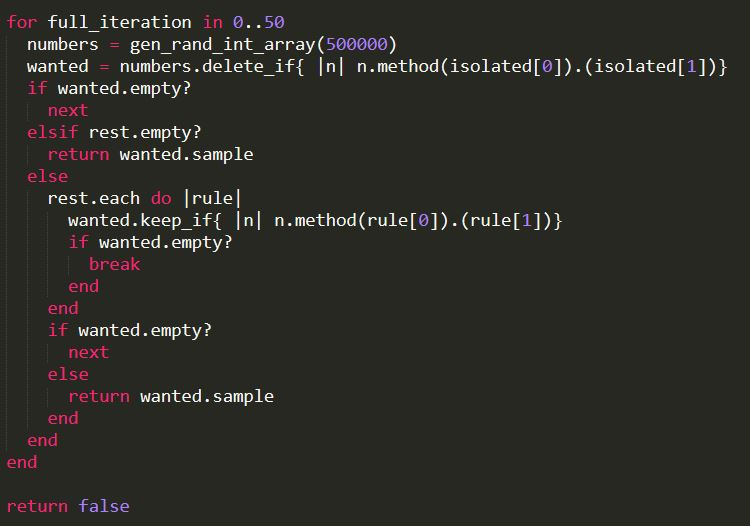
\includegraphics[width=\linewidth]{screenshots/code-gen-int-pre_divisible_keep_if}
\caption{caption for image, shown below image}
\label{fig:code1}
\end{figure}
Figure \ref{fig:code1} shows some savage code

	
\begin{table}[h!]
\centering
\caption{Caption for the table.}
\label{tab:table1}
\begin{tabular}{ccc}
\toprule
Some & actual & content\\
\midrule
prettifies & the & content\\
as & well & as\\
using & the & booktabs package\\
\bottomrule
\end{tabular}
\end{table}

\begin{table}
\caption{Data Types Supported}
\label{tab:datatypessupported}
    \begin{tabular}{|l|}
        \hline
        Data Type \\ \hline
        Integer   \\ 
        Float     \\ 
        String    \\
        \hline
    \end{tabular}
\end{table}

\begin{table}
\caption{Integer and Float Validations Supported}
\label{tab:integersupported}
    \begin{tabular}{|l|}
        \hline
        Validation               \\ \hline
        Blank                    \\ 
        Inclusion                \\ 
        Exclusion                \\ 
        Greater Than             \\ 
        Greater Than or Equal To \\ 
        Equal To                 \\ 
        Less Than or Equal To    \\ 
        Less Than                \\ 
        Other Than               \\ 
        Divisible                \\
        \hline
    \end{tabular}
\end{table}

\begin{table}
\caption{String Validation Supported}
\label{tab:stringsupported}
    \begin{tabular}{|l|}
        \hline
        Validation     \\ \hline
        Blank          \\ 
        Inclusion      \\ 
        Exclusion      \\ 
        Minimum Length \\ 
        Maximum Length \\ 
        Exact Length   \\ 
        Format         \\
        \hline
    \end{tabular}
\end{table}